
\section{Introduction}

The transition from static language models to autonomous agents marks a pivotal shift in artificial intelligence, enabling systems to handle complex, dynamic tasks through iterative reasoning and tool use~\citep{cheng2024exploring,tao2024survey,gao2025survey,fang2025comprehensive}. 
To facilitate continuous improvement without expensive parameter retraining, \textbf{procedural memory}—which internalizes ``how-to'' knowledge from past interactions—has emerged as a critical substrate for agent evolution~\citep{zhang2025survey,xu2025mem}. 
By accumulating high-quality problem-solving experiences, agents can leverage prior successes to navigate novel scenarios, theoretically reducing redundant trial-and-error and circumventing local optima~\citep{wang2025mirix,chen2025swe} (as shown in Figure~\ref{fig:example}).

However, despite the promise of memory-augmented agents, current frameworks predominantly suffer from a \textbf{``passive accumulation''} paradigm. 
Prevailing approaches typically treat memory as a static append-only archive, storing raw, trajectory-level interactions~\citep{zheng2023synapse,hu2024hiagent} or generalized workflows~\citep{tang2025agentkb,liu-etal-2025-contextual}. 
This introduces two fundamental limitations. 
First, the \textbf{granularity mismatch}: retaining entire trajectories introduces significant contextual noise (e.g., irrelevant observations), which dilutes the agent's attention on critical reasoning logic during retrieval. 
Second, the \textbf{lack of evolution}: agents operate in non-stationary environments where task distributions shift and their own capabilities improve. Without a mechanism to prune obsolete or ineffective entries, the memory pool inevitably degrades into a mixture of valid insights and ``toxic'' noise, leading to negative transfer and hallucinations~\citep{xiong2025memory}.

\begin{figure*}
    \centering
    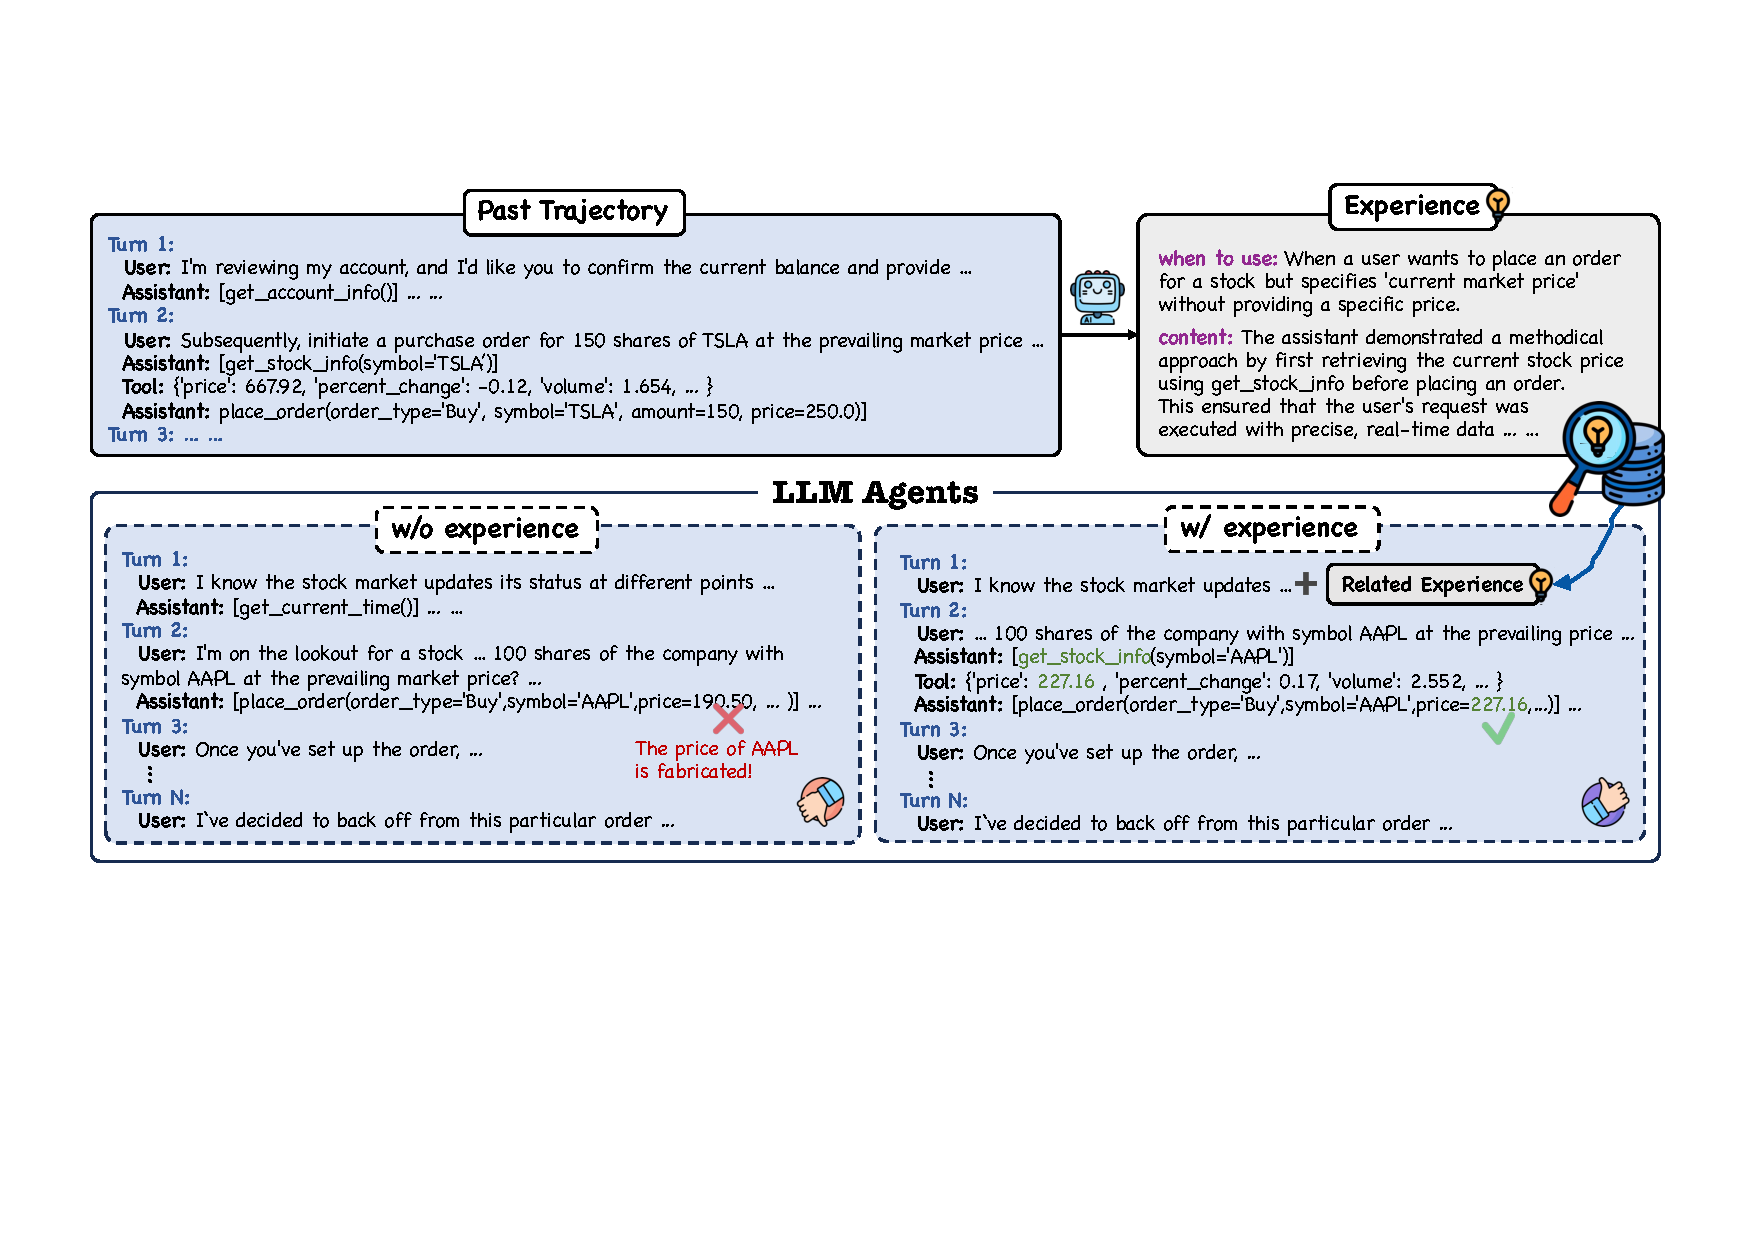
\includegraphics[width=1\linewidth]{figures/example.pdf}
    \caption{Example of how agents complete one stock trading task with and without past experience.}\label{fig:example}
\end{figure*}

To address these challenges, we propose \textbf{\ours} (\textit{Remember Me, Refine Me}), a dynamic framework that shifts the paradigm from passive storage to \textbf{feedback-driven experience evolution}. 
Instead of indiscriminately archiving trajectories, {\ours} employs a \textbf{contrastive distillation strategy}. By analyzing the divergence between successful and failed attempts, the system isolates the \textbf{pivotal decision points}—the specific strategic moves that differentiate high-quality outcomes from suboptimal ones—thereby maximizing the signal-to-noise ratio of stored knowledge.
Furthermore, to combat memory degradation, {\ours} introduces a \textbf{utility-based evolutionary mechanism}. 
Treating the memory pool as a living ecosystem, our framework quantitatively tracks the utility of each experience during reuse. It autonomously reinforces validated strategies while pruning entries that fail to contribute to task success, ensuring the memory pool continuously adapts to changes in the problem and the agent's development.

Our extensive experiments on BFCL-V3 and AppWorld benchmarks demonstrate that {\ours} establishes a new state-of-the-art for memory-augmented agents. 
Most notably, our results reveal that memory quality can substitute for model scale: \textbf{{\ours} enables a Qwen3-8B model to outperform a parameter-heavier Qwen3-14B baseline (without memory)}, achieving average gains of 10.65\% in Avg@4. 
These findings suggest that a self-evolving memory mechanism offers a computationally efficient pathway for agent evolution, narrowing the gap between small and large models through strategic experience management.

In summary, our contributions are as follows:
\begin{itemize}[leftmargin=12pt,topsep=2pt,itemsep=-2pt]
    \item We propose \textbf{\ours}, a dynamic framework that evolves procedural memory through \textbf{contrastive experience distillation}, extracting keypoint-level insights to resolve the granularity mismatch inherent in trajectory-based approaches.
    \item We introduce a \textbf{utility-based evolutionary mechanism} that establishes a quantitative feedback loop for memory management, enabling the agent to autonomously maintain a high-quality, adaptive memory pool by pruning ineffective entries.
    \item We design a context-adaptive reuse strategy that incorporates \textbf{failure-aware reflection}, allowing agents to dynamically adjust their reasoning paths when historical experiences do not perfectly align with new tasks.
    \item Empirical results confirm that {\ours} significantly enhances agent performance, allowing smaller models to surpass larger baselines and demonstrating a scalable approach to lifelong agent learning.
\end{itemize}
